\documentclass[oneside,final,14pt,a4paper]{extreport}

\usepackage{tempora} % Times New Roman alike font  

\usepackage{vmargin}
\setpapersize{A4}
\setmarginsrb{2.5cm}{2cm}{2cm}{2cm}{0pt}{10mm}{0pt}{13mm}
\usepackage{setspace}
\setstretch{1.5}
\usepackage{indentfirst}
\parindent=1.25cm

%%%%% ADDED TO SUPPORT TT BOLD FACES %%%%
\DeclareFontShape{OT1}{cmtt}{bx}{n}{<5><6><7><8><9><10><10.95><12><14.4><17.28><20.74><24.88>cmttb10}{}
\renewcommand{\ttdefault}{pcr}
%%%%% END %%%%%%%%%%%%%%%%%%%%%%%%%%%%%%% 

\usepackage{atbegshi,picture}
% \usepackage[T1, T2A]{fontenc}
\usepackage[utf8]{inputenc}

\usepackage[russian]{babel}

\usepackage{hyphenat}

\usepackage[default]{droidserif}
\usepackage[defaultsans]{droidsans}

\usepackage[babel=true]{microtype}
\usepackage[backend=biber,style=ieee,autocite=inline]{biblatex}
\bibliography{ref.bib}
\DefineBibliographyStrings{english}{%
  bibliography = {References},}
\usepackage{blindtext}

\usepackage{pdfpages}
\newenvironment{bottompar}{\par\vspace*{\fill}}{\clearpage}
\usepackage{amsmath,amsfonts,amsopn}
\usepackage{url}
\usepackage{amsthm}
\newtheorem{theorem}{Theorem}
\newtheorem{corollary}{Corollary}
\newtheorem{lemma}{Lemma}
\newtheorem{proposition}{Proposition}
\theoremstyle{definition}
\newtheorem{definition}{Definition}
\theoremstyle{remark}
\newtheorem*{remark}{Remark}
\theoremstyle{remark}
\newtheorem*{example}{Example}
\DeclareMathOperator{\Exp}{Exp}

\usepackage{float}
\usepackage{graphicx}
\graphicspath{{figs/}} %path to images
\usepackage{array}
\usepackage{multirow,array}
\usepackage{caption}
\usepackage{subcaption}
\usepackage{hyperref}
\hypersetup{
	colorlinks=true,
	linkcolor=black,
	citecolor=black,
	urlcolor=black
}
\usepackage{paralist}
\usepackage{listings}
\usepackage{zed-csp}
\usepackage{fancyhdr}
\usepackage{csquotes}
\usepackage{color}
% \usepackage{anyfontsize}
% \usepackage{mathptmx}
% \usepackage{t1enc}

\usepackage{chngcntr}
\usepackage{upgreek}
\usepackage{bm}
\usepackage{booktabs}
\usepackage{multirow}
\usepackage{longtable}
\usepackage{forest}
% \usepackage{lmodern}

\usepackage[font=singlespacing, labelfont=bf]{caption}
%Hints
\newcommand\pic[1]{(Fig. \ref{#1})} %Ref on figure
\newcommand\tab[1]{(Tab. \ref{#1})} %Ref on table

\setlength{\headheight}{32.0976pt}
\usepackage{enumitem}
\newlist{inlinelist}{enumerate*}{1}
\setlist*[inlinelist,1]{%
  label=(\arabic*),
}

% \setcounter{secnumdepth}{4}
\captionsetup[table]{labelfont={normalfont}, name={Таблица}, labelsep={newline}}
\setlength{\parindent}{2em} 
\DeclareCaptionLabelSeparator{figSep}{.\quad}
\captionsetup[figure]{labelfont={normalfont},justification=raggedright, singlelinecheck=false, name={Рисунок}, labelsep=period}

\usepackage{titlesec}
\titleformat{\chapter}[hang]
  {\normalfont\huge\bfseries} % Format for the whole title block
  {\thechapter.}              % The label (chapter number + period)
  {1em}                       % Horizontal space between number and title
  {}                          % Code before the title text (leave empty)
% \titleformat{\section}[hang]{\fontsize{20}{24}\selectfont\filcenter}{}{1em}{}
% \titleformat{\subsection}[hang]{\itshape}{\Alph{subsection}.}{1em}{}[]
% \titleformat{\subsubsection}[runin]{\itshape}{\arabic{subsubsection})}{1em}{}[$:$]
% \titlespacing{\subsubsection}{1em}{1em}{1em}
% \titleformat{\paragraph}[runin]{\itshape}{\alph{paragraph})}{1em}{}[$:$\quad]
% \titlespacing{\paragraph}{2em}{1em}{1em}

\usepackage{placeins} % for \FloatBarrier

\pagestyle{fancyplain}

% remember section title
\renewcommand{\chaptermark}[1]%
{\markright{\thechapter\ #1}{}}

% subsection number and title
\renewcommand{\sectionmark}[1]%
	{\markright{\thesection\ #1}}

\rhead[\fancyplain{}{\bf\leftmark}]%
      {\fancyplain{}{\bf\thepage}}
\lhead[\fancyplain{}{\bf\thepage}]%
      {\fancyplain{}{\bf\rightmark}}
\cfoot{} %bfseries


\newcommand{\dedication}[1]
   {\thispagestyle{empty}
     
   \begin{flushleft}\raggedleft #1\end{flushleft}
}

% \usepackage{tocloft}
% \renewcommand{\contentsname}{Содержание}
% \renewcommand{\cfttoctitlefont}{\LARGE\bfseries}

\usepackage{fontspec}
\setmainfont{Times New Roman}

\begin{document}

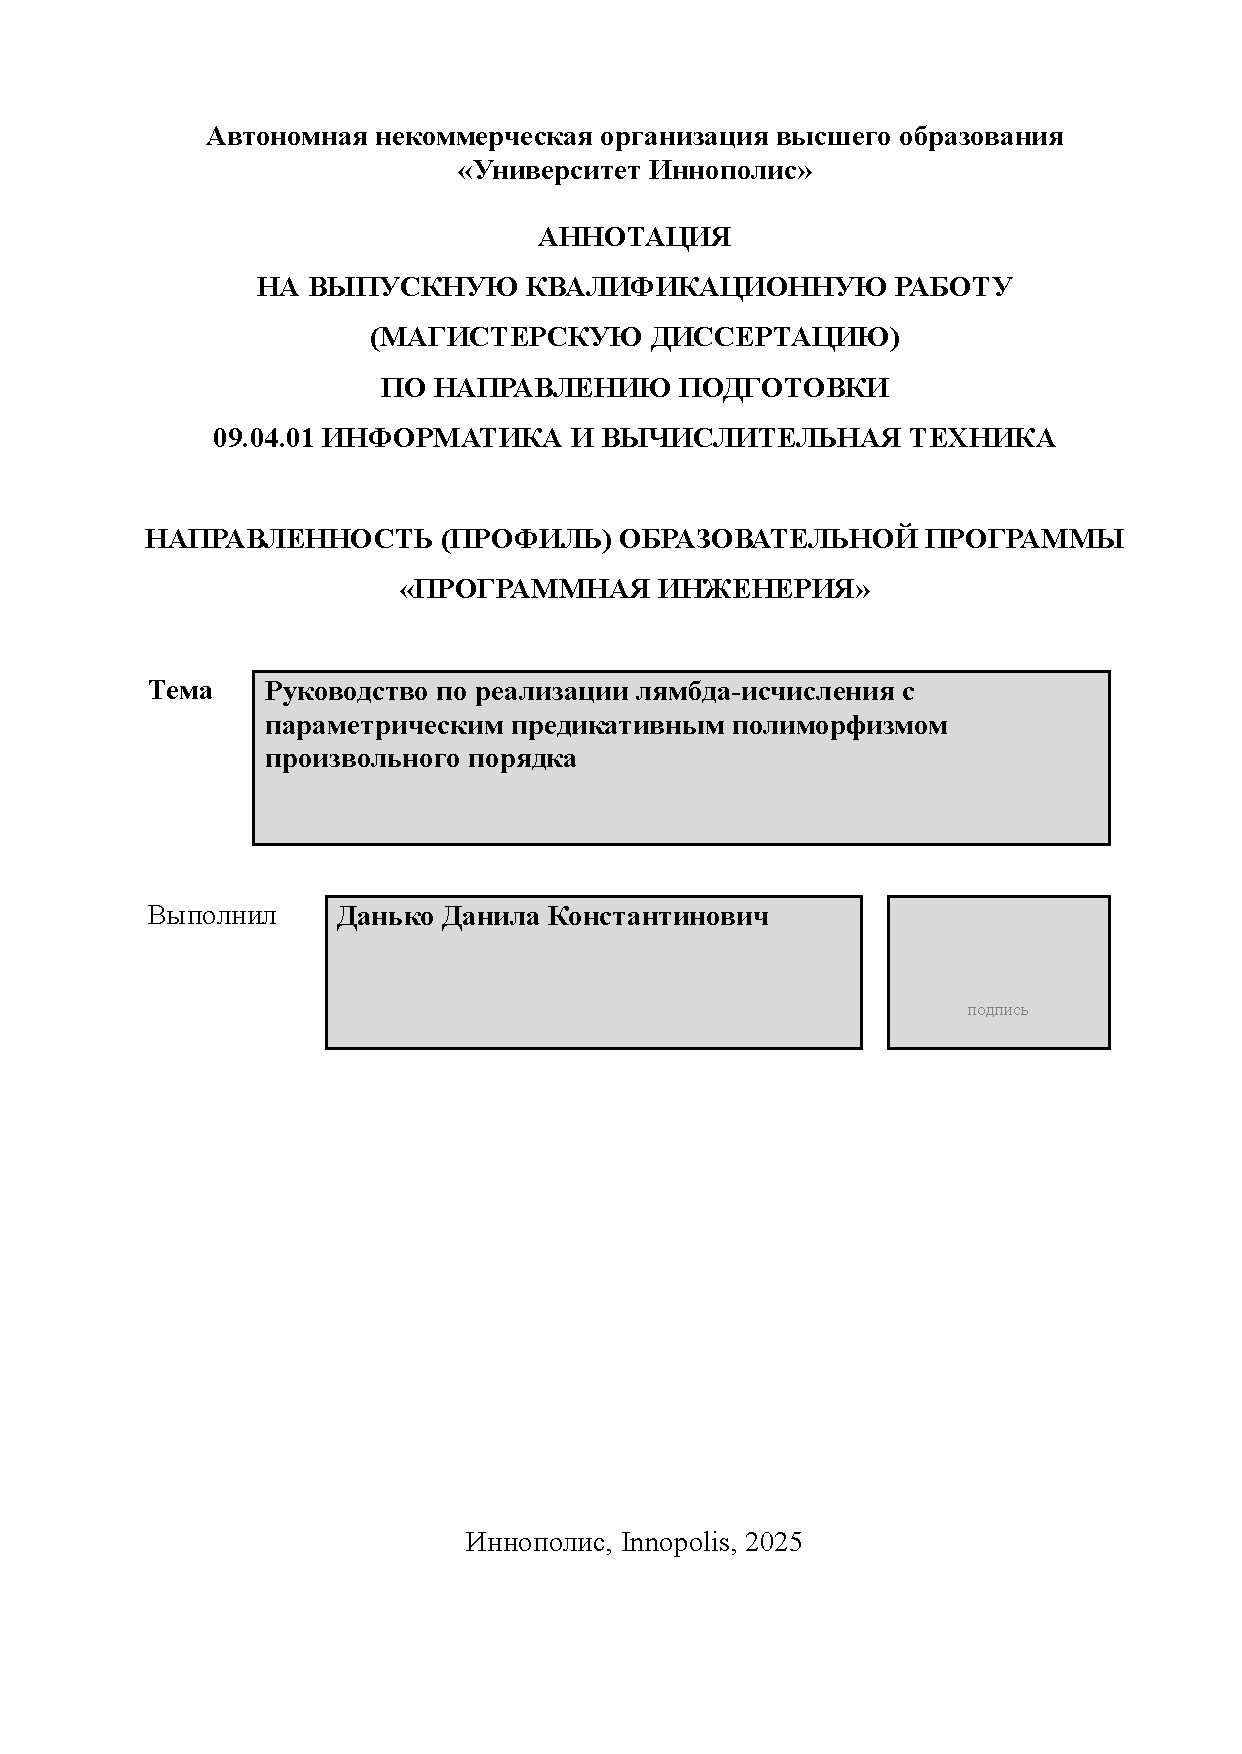
\includepdf[noautoscale,offset=75 -75,pages=-]{title.pdf}
\tableofcontents
% \listoftables
% \listoffigures
% \newpage

\selectlanguage{russian}
\chapter*{АННОТАЦИЯ}
\addcontentsline{toc}{chapter}{Аннотация}

\section*{Общая характеристика работы}

Настоящая диссертация посвящена проектированию и реализации \texttt{Arralac} — небольшого функционального языка программирования и сопутствующего ему компилятора. Основная цель проекта — преодолеть педагогический разрыв между сложной академической теорией систем типов и практикой реализации современных компиляторов. Работа не претендует на научную новизну, а фокусируется на применении известных, но передовых инженерных подходов для создания прозрачного, модульного и интерактивного инструмента, предназначенного для изучения внутреннего устройства компилятора.

Центральный тезис работы заключается в том, что сфокусированная, современная и интерактивная реализация, сознательно отходящая от старых алгоритмических моделей, может служить более эффективным средством обучения, чем изолированное изучение фундаментальных научных статей или исходного кода промышленных компиляторов.

Работа представляет собой полный цикл разработки: от теоретического обоснования и проектирования архитектуры до реализации, тестирования и анализа полученной системы. Особое внимание уделяется двум ключевым аспектам современной инженерии компиляторов: архитектуре вывода типов на основе ограничений (constraint-based) и представлению Абстрактного синтаксического дерева (АСД) с помощью паттерна «Растущие деревья» (Trees That Grow).

\section*{Актуальность темы}

Продвинутые системы типов являются краеугольным камнем современного функционального программирования. Одной из таких мощных возможностей является \textbf{полиморфизм произвольных рангов} (arbitrary-rank polymorphism), который позволяет функциям принимать в качестве аргументов другие полиморфные функции. Эта возможность лежит в основе реализации таких продвинутых языковых средств, как обобщённые алгебраические типы данных (GADT), программирование на уровне типов и сложные формы обобщённого программирования.

\enlargethispage{\baselineskip}
Теоретические основы для реализации этой функции в практическом компиляторе были заложены в основополагающей статье Пейтона Джонса и др. «Practical type inference for arbitrary-rank types» \cite{jones-practical-2007}. Самой известной реализацией этих идей является компилятор языка Haskell — Glasgow Haskell Compiler (GHC) \cite{ghc-site-2025}. Для многих разработчиков, включая автора данной работы, внутреннее устройство GHC представляет собой вершину компиляторных технологий — «достаточно развитую технологию», которая может казаться магией.

Несмотря на наличие как фундаментальной теории, так и промышленной реализации, существует значительный педагогический разрыв. Начинающие разработчики языков и студенты сталкиваются с крутой кривой обучения при попытке понять, как элегантная теория полиморфизма произвольных рангов преобразуется в практический код. Этот разрыв обусловлен несколькими факторами:
\begin{itemize}
\item \textbf{Академическая литература}, включая \cite{jones-practical-2007}, представляет теоретически плотную систему, построенную на сложном взаимодействии \textbf{субсумпции} (subsumption), \textbf{глубокой сколемизации} (deep skolemization) и \textbf{двунаправленной проверки типов} (bidirectional checking). Хотя система формально корректна \cite{practical-type-inference-proofs}, описание алгоритма \textbf{«жадного» объединения} (eager unification) в статье опускает множество практических инженерных деталей, необходимых для построения надёжной системы.
\item \textbf{Исходный код GHC}, будучи бесценным ресурсом, представляет собой огромную, высокооптимизированную промышленную систему. Его современная архитектура вывода типов, \textbf{основанная на ограничениях} (constraint-based), является значительной эволюцией по сравнению с «жадной» моделью, описанной в основополагающих статьях. Это затрудняет прослеживание связи между теорией и реализацией для новичка. Современные аналоги, такие как MicroHs \cite{augustsson-microhs-2024, augustss-microhs-2025}, также являются крупными проектами.
\item \textbf{Существующие учебные компиляторы} для Haskell, такие как Hugs \cite{hugs-haskell}, устарели или не включают эти современные архитектурные паттерны, оставляя студентов без моста от базовых принципов к современному состоянию дел.
\end{itemize}

Таким образом, возникает очевидная потребность в ресурсе, который преодолевает этот разрыв, — «промежуточном звене», более конкретном, чем статья, но более сфокусированном и доступном, чем полноценный промышленный компилятор, и который явно демонстрирует архитектурную эволюцию от «жадной» модели к выводу типов на основе ограничений.

\section*{Цель, предмет и объект исследования}
Основной \textbf{целью} данной работы является создание дидактического компилятора \texttt{Arralac}, который служит учебным пособием по реализации полиморфизма произвольных рангов с использованием современных архитектурных практик.

\textbf{Объектом} исследования является процесс проектирования и реализации компиляторов для функциональных языков программирования с продвинутыми системами типов.

\textbf{Предметом} исследования является архитектура и реализация компилятора \texttt{Arralac} как дидактического инструмента для изучения полиморфизма произвольных рангов, в частности, модель вывода типов на основе ограничений, паттерн «Растущие деревья» и интеграция с инструментами интерактивной разработки.

Для достижения поставленной цели были сформулированы следующие \textbf{задачи}:
\begin{enumerate}
\item Реализовать ключевые алгоритмы двунаправленной системы вывода типов для полиморфизма произвольных рангов, включая субсумпцию и глубокую сколемизацию, в ясной и модульной манере, пригодной для образовательных целей.
\item Продемонстрировать на практике, что модель вывода типов, основанная на ограничениях (разделение генерации и решения), служит более понятным педагогическим инструментом для объяснения вывода типов, чем модель «жадного» объединения, представленная в фундаментальной литературе.
\item Использовать протокол языкового сервера (LSP) для создания интерактивной среды разработки, которая делает поведение и результаты конвейера вывода типов языка прозрачными и исследуемыми, превращая абстрактные правила в конкретную обратную связь.
\item Создать общедоступный репозиторий с документированным исходным кодом \cite{deemp-arbitrary-rank-tutorial} в качестве ресурса для сообщества для обучения и экспериментов.
\end{enumerate}

\section*{Методы исследования}
Для решения поставленных задач в работе использовался комплексный подход, включающий следующие методы:
\begin{itemize}
\item \textbf{Теоретические методы:} анализ и синтез научно-технической литературы по теориям систем типов, алгоритмам вывода типов и архитектуре компиляторов; изучение основополагающих работ (в частности, \cite{jones-practical-2007}) и современных исследований в области.
\item \textbf{Методы системного проектирования:} применение модульного подхода и конвейерной архитектуры для декомпозиции сложной задачи компиляции на управляемые этапы (парсинг, переименование, проверка типов, решение ограничений, оценка).
\item \textbf{Методы программной инженерии:} реализация системы на языке функционального программирования Haskell; применение современных архитектурных паттернов, таких как «Растущие деревья» (Trees That Grow), для создания расширяемого и типобезопасного АСД; использование системы управления зависимостями Nix для обеспечения воспроизводимости сборки.
\item \textbf{Эмпирические методы:} разработка и использование набора целевых тестовых примеров для верификации корректности реализации ключевых механизмов системы типов (обработка полиморфизма высших рангов, обнаружение утечки сколемов); ручное тестирование интерактивных функций языкового сервера.
\end{itemize}

\section*{Научные и практические результаты}
В ходе выполнения диссертационной работы были получены следующие основные результаты:
\begin{enumerate}
\item \textbf{Разработан и реализован компилятор \texttt{Arralac}}, представляющий собой функциональный, хорошо структурированный и нетривиальный учебный проект. Система успешно компилирует и выполняет программы на языке с полиморфизмом произвольных рангов.
\item \textbf{Продемонстрирована эффективность двухфазной архитектуры вывода типов.} В отличие от «жадной» модели из \cite{jones-practical-2007}, \texttt{Arralac} разделяет генерацию ограничений и их решение. Это позволило создать более модульную систему, где логика проверки типов и логика унификации полностью разделены, а также заложить основу для более качественной диагностики ошибок.
\item \textbf{Реализовано представление АСД с использованием паттерна «Растущие деревья».} Данный подход обеспечил типобезопасное добавление аннотаций (таких как выведенные типы) на разных стадиях конвейера компиляции, что является необходимым условием для создания современных инструментов разработки и делает эволюцию структуры данных наглядной.
\item \textbf{Создан интерактивный инструментарий на основе LSP.} Реализация языкового сервера, который предоставляет информацию о выведенных типах при наведении курсора и сообщает об ошибках в реальном времени, превращает компилятор из «чёрного ящика» в интерактивный инструмент для изучения его работы.
\item \textbf{Создан общедоступный образовательный ресурс.} Весь исходный код проекта, включая подробные комментарии, опубликован в открытом доступе и снабжён средствами для быстрой и воспроизводимой установки, что позволяет использовать его в качестве учебного пособия.
\end{enumerate}

\section*{Структура и краткое содержание работы}

Диссертация состоит из введения, четырёх глав, заключения и списка литературы.

\textbf{Во введении} обосновывается актуальность темы, определяется проблема педагогического разрыва между теорией и практикой в области компиляторов, формулируются цели и задачи исследования, а также описывается вклад работы в решение этой проблемы.

\textbf{В первой главе, «Обзор литературы»,} представлены теоретические основы работы. Глава прослеживает эволюцию полиморфных систем типов: от фундаментальных ограничений Простого типизированного лямбда-исчисления, через теоретический идеал Системы F и практический компромисс Хиндли-Милнера, к «пробелу N-го ранга» (Rank-N gap). Завершается глава детальным обзором двунаправленного подхода для типов произвольных рангов, предложенного в \cite{jones-practical-2007}, который является теоретическим ядром диссертации.

\textbf{Во второй главе, «Проектирование и методология»,} подробно описывается архитектура и реализация языка \texttt{Arralac}. Рассматривается полный конвейер компиляции. Особый акцент сделан на ключевых архитектурных решениях: выборе паттерна «Растущие деревья» для представления АСД, а также на сознательном отходе от «жадной» унификации в пользу двухфазной архитектуры проверки типов на основе ограничений, вдохновлённой GHC. Описывается использование уровней (TcLevel) для контроля области видимости полиморфных переменных.

\textbf{В третьей главе, «Реализация и результаты»,} демонстрируется практическая реализация спроектированной системы на языке Haskell. Описывается структура данных для АСД и её инстанцирование для разных фаз компиляции. Детально рассматривается конвейер вывода типов: генерация ограничений, их решение отдельным модулем-решателем и финализация (зонкинг). Глава завершается демонстрацией работы компилятора на конкретных примерах: успешная проверка типов для программы с полиморфизмом высших рангов, корректное обнаружение ошибки (утечка сколема) и работа интерактивных инструментов (LSP).

\textbf{В четвёртой главе, «Анализ и обсуждение»,} проводится критический анализ полученной системы. Оценивается, насколько успешно выбранные архитектурные решения (вывод типов на ограничениях, «Растущие деревья») способствовали достижению педагогических целей. Обсуждаются компромиссы принятых решений, а также качественные характеристики системы, такие как модульность и анализируемость. В заключительной части главы определяются ограничения текущей реализации (отсутствие let-генерализации, неунифицированный решатель) и намечаются конкретные направления для будущих исследований.

\textbf{В заключении} подводятся итоги работы, делается вывод о достижении поставленных целей. Пересматривается центральный тезис в свете полученных результатов и подтверждается, что современная, сфокусированная реализация является эффективным средством для демистификации сложных компиляторных технологий. Намечаются дальнейшие шаги по развитию проекта.

% \setcounter{page}{8}
% set manually the number, from which Chapter 1 starts!
% Why do we put 7 in this case?
% Title page - page 1
% Contents - page 2, page 3
% List of tables - page 4
% List of figures - page 5
% Abstract - page 6
% Chapter 1 - page 7
% In your thesis the counter number can be different, please count carefully and insert the corresponding number.

% \include{chapters/chapter1}
% \include{chapters/chapter2}
% \include{chapters/chapter3}
% \include{chapters/chapter4}
% \include{chapters/chapter5}
% \include{chapters/chapter6}


%% REFERENCES
{\sloppy
  \printbibliography[heading=bibintoc,title={Список литературы}]
}
%\include{chapters/appex}
\end{document}